% プロジェクト学習中間報告書書式テンプレート ver.1.0 (iso-2022-jp)

% 両面印刷する場合は `openany' を削除する
\documentclass[openany,11pt,papersize]{jsbook}

% 報告書提出用スタイルファイル
%\usepackage[final]{funpro}%最終報告書
\usepackage[middle]{funpro}%中間報告書

% 画像ファイル (EPS, EPDF, PNG) を読み込むために
\usepackage[dvipdfmx]{graphicx,color}

% ここから -->
\usepackage{calc,ifthen}
\newcounter{hoge}
\newcommand{\fake}[1]{\whiledo{\thehoge<70}{#1\stepcounter{hoge}}%
  \setcounter{hoge}{0}}
% <-- ここまで 削除してもよい

% 年度の指定
\thisYear{2016}

% プロジェクト名
\jProjectName{使ってもらって学ぶフィールド指向システム・デザイン}

% [簡易版のプロジェクト名]{正式なプロジェクト名}
% 欧文のプロジェクト名が極端に長い(2行を超える)場合は、短い記述を
% 任意引数として渡す。
%\eProjectName[Making Delicious curry]{How to make delicious curry of Hakodate}
\eProjectName{Field Oriented System Design Learning by Users' Feedback}


% <プロジェクト番号>-<グループ名>
\ProjectNumber{03-A}

% グループ名
\jGroupName{町内会グループ}
\eGroupName{Nighborhood Association Group}

% プロジェクトリーダ
\ProjectLeader{1014237}{伊藤泰斗}{Taito~Ito}

% グループリーダ
\GroupLeader  {1014120}{永井陽太}{Youta~Nagai}

% メンバー数
\SumOfMembers{5}
% グループメンバ
\GroupMember  {1}{1014237}{伊藤泰斗}{Taito~Ito}
\GroupMember  {2}{1014120}{永井陽太}{Youta~Nagai}
\GroupMember  {3}{1014253}{横山新}{Taro~Hokkai }
\GroupMember  {4}{1014231}{森島帆南}{Honami~Morishima}
\GroupMember  {5}{1014059}{船木綾香}{Ayaka~Funaki}

% 指導教員
\jadvisor{伊藤恵,南部美砂子,奥野拓,木塚歩,原田泰}
% 複数人数いる場合はカンマ(,)で区切る。カンマの前後に空白は入れない。
\eadvisor{Kei~Ito,Misako~Nambu,Taku~Okuno,Ayumi~Kiduka,Yasushi~Harada}

% 論文提出日
\jdate{2016年7月27日}
\edate{July~27, 2016}

\begin{document}
%
% 表紙
\maketitle

%前付け
\frontmatter

% 和文概要
\begin{jabstract}
\fake{ここに日本語の概要を書きます。}
% 和文キーワード
\begin{jkeyword}
キーワード1, キーワード2, キーワード3, キーワード4, キーワード5
\end{jkeyword}
\bunseki{伊藤泰斗}
\end{jabstract}

%英語の概要
\begin{eabstract} Abstract in English.
\fake{you should write your English abstract in one page. }
% 英文キーワード
\begin{ekeyword}
Keyrods1, Keyword2, Keyword3, Keyword4, Keyword5
\end{ekeyword}
\bunseki{伊藤泰斗}
\end{eabstract}


\tableofcontents% 目次


\mainmatter% 本文のはじまり

%背景
\chapter{背景}

\section{陣川町について}
陣川町は北海道函館市にある町である。陣川町には「陣川あさひ町会(以降、町会とする)」がある。町会は陣川町の1,200世帯中約1,000世帯が加入している。夏には参加者が約1,000人にもなる納涼まつりや冬にはウィンターフェスティバルを行うなど積極的に活動し
ている。また、これらのイベント情報を多くの人に知ってもらいたいため町会役員がFacebookとLINE@を使い発信している。しかし、積極的にイベントを開催する反面で様々な問題を抱えている。
\bunseki{船木綾香}

\section{町会が抱える問題}
町会のイベントを開催する上での問題点は主に以下の6つである。
\begin{itemize}
    \item FacebookやLINE@ではイベントに関するお知らせはできるが、開催予定のイベントを一覧で見れない。
    \item イベントの情報が決まった際にFacebookとLINE@に同一の内容を発信する手間がかかる。
    \item 町民のイベント申し込み方法が電話、FAX、メールの3つあり、イベント参加者の管理に手間がかかる。
    \item Facebookでは個人情報が漏れてしまうため参加申し込みができない。
    \item 役員だけで共有したい情報を町民に知られずに共有することがFacebookやLINE@ではでできない。
    \item イベント当日が悪天候の場合、参加者全員に対してイベントの中止、延期などの連絡を迅速に行うことができない。
\end{itemize}
このように、町会はイベントを開催する上で様々な問題を抱えている。
\bunseki{船木綾香}


%目的
\chapter{目的}
​
\section{このグループの目的}%例:レビュー内容
% 必要ならここに大見出しの内容
%必要なら下のsubsectionを用いて小見出しをつかう
%\subsection{ここに小見出し}%:発表技法について
本グループでは「陣川あさひ町会のイベント開催に関する問題を解決するサービスの提供をする」ことを目的と設定した。前述の通り、陣川あさひ町会ではイベントを開催する上でさまざまな問題がある。そこで本グループではそれらの問題を解決するアプリケーションを開発する。
\bunseki{船木綾香}


%開発準備
\chapter{開発準備}

\section{開発に利用したツールとその経緯}%例:レビュー内容
%必要ならここに大見出しの内容
%必要なら下のsubsectionを用いて小見出しをつかう
\subsection{Monaca}%:発表技法について
iOSとAndroidの両方のプラットフォームでアプリケーションを使いたいという町会の要望を叶えるために, HTML5ハイブリッドアプリを開発することとした. iOSとAndroidには, 「WebView」と呼ばれるブラウザの機能を持つコンポーネントが組み込まれている\cite{book_about_monaca}. HTML5ハイブリッドアプリとは, 「WebView」にHTMLとCSS, JavaScriptを用いて開発するアプリケーションである\cite{book_about_monaca}. また, HTML5ハイブリッドアプリの開発ツールのなかからMonacaを選択した. MonacaはCordovaというオープンソースのフレームワークを利用している\cite{book_about_monaca}. また, MonacaにはMonacaクラウドIDE, Monaca Localkit, Monaca CLIの3種類の開発環境が存在する\cite{book_about_monaca}. MonacaクラウドIDEは, インターネットクラウド上で開発するため個人の開発環境に依存しない\cite{book_about_monaca}. Monaca Localkitは, MonacaクラウドIDEとは異なり, 各メンバごとにローカルでの開発を可能とする\cite{book_about_monaca}. Monaca CLIは, MonacaクラウドIDEが提供するサービスを, コマンドライン形式で利用することを可能にする\cite{book_about_monaca}. いずれの開発環境においても, Monacaデバッカーを用いて, デバックを行う(図\ref{fig:image_monaca}).

\begin{figure}[h]
  \begin{center}
  %\begin{flushleft}
    \begin{tabular}{c}

      % 1
      \begin{minipage}{0.7\hsize}
        \begin{center}
\includegraphics[width=10cm]{monaca_overview.png}
          \hspace{1cm} %(a)観光スポットの紹介
        \end{center}
      \end{minipage}

    \end{tabular}
    \caption{Monacaでの開発イメージ\cite{monaca_debugger}}
    \label{fig:image_monaca}
  \end{center}
  %\end{flushleft}
\end{figure}

\subsection{ニフティクラウド mobile backend}%:発表技法について
本アプリケーションの各情報を保存する場所として, mBaaSの1つであるニフティクラウド mobile backend(以下, NCMBとする)を使用した. 使用した理由として, 以前このサービスを利用したことがあること, 他のmBaaSと比べて無料で利用可能な機能多いことが挙げられる. mBasSとは, サーバーの開発, 運用を必要とせずユーザから直接見えない部分の機能をアプリケーションに実装することを可能にするサービスである\cite{about_mbaas}. NCMBは, プッシュ通知, 会員管理と認証, SNS連携などの機能\cite{price_mbaas}を提供しているサービスである(図\ref{fig:image_mbaas}).

\begin{figure}[htbp]
%\begin{flushleft}
  \begin{center}
    \begin{tabular}{c}

      % 1
      \begin{minipage}{0.7\hsize}
        \begin{center}
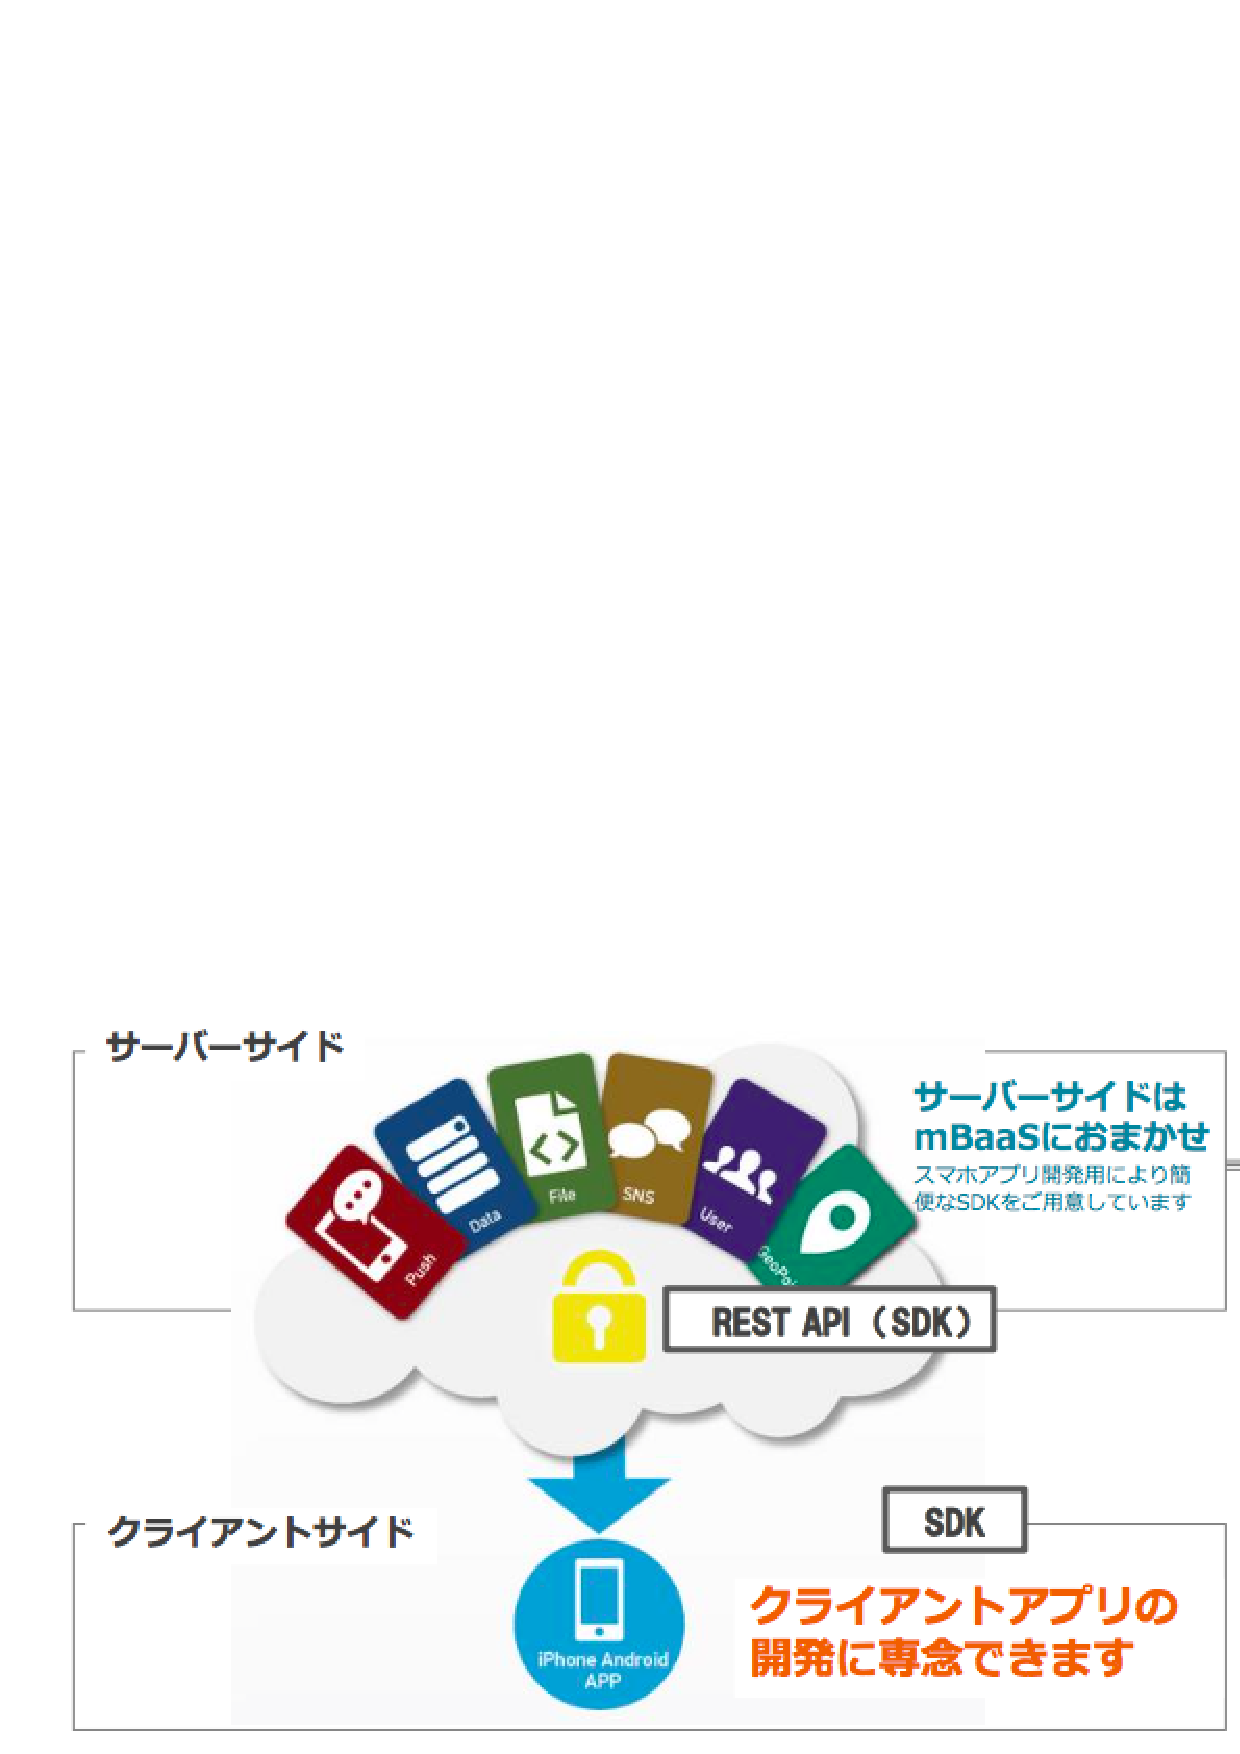
\includegraphics[width=10cm]{ncmb_overview.png}
          \hspace{1cm} %(a)観光スポットの紹介
        \end{center}
      \end{minipage}

    \end{tabular}
    \caption{ニフティクラウド mobile backendのサービス内容\cite{intro_mbaas}}
    \label{fig:image_mbaas}
  \end{center}
  %\end{flushleft}
\end{figure}


\subsection{Git/GitHub}%:発表技法について
ソースコードのバージョン管理ツールとして, Git/GitHubを使用した. Gitはファイルの変更履歴をリポジトリと呼ばれる場所に保存する. そのため, 一度編集したファイルを過去の状態に復元することや, 編集箇所を表示することが可能となる\cite{book_about_github}. リポジトリの種類は, メンバのローカルPC内に存在するローカルリポジトリと, インターネット上に存在するリモートリポジトリの2種類である\cite{monkey_git}. リモートリポジトリでは, 各メンバのファイルの変更履歴を保存し, 共有する事が可能である. GitHubは, リモートリポジトリを提供するサービスの1つである. これにより, 複数のメンバで同時に開発を進めることが可能となった.

\subsection{Slack}%:発表技法について
チーム内のコミュニケーションツールとして, Slackというチャットツールを使用した. Slackには数多くの特徴や機能が備わっているが, 本プロジェクトでは以下の2個の機能を主に使用した. 1つ目は, 一つのteamに対して複数のチャンネルを作成することができる機能である. Slackはまず最初にteamというものを作成する. これは, teamの名前は"2016プロジェクト03"など, 団体名やプロジェクト名で名付ける. その後, 議題ごとに"\#report"や"\#design"などとチャンネルを作成することが出来る. これらの機能のお陰で, 1つの話題について見逃すこと無く, 集中して話し合うことができた. また, ファイルやリンクの共有についても同様に, チャンネルごとに分けて行うことができた. 2つ目は, GitHubなどの他のサービスと連携することができる機能である. 連携先のGitHubに何らかの変更が生じた時に, 指定したチャンネルに通知が来るように設定した. この機能のお陰でアプリケーションや報告書に変更があった場合に, グループメンバ全員が進捗の把握をしやすい環境を整えられた.

\subsection{Redmine}%:発表技法について
タスク管理ツールとして前期は, Redmineというオープンソースソフトウェアを使用した. Redmineでは, 発生したタスクごとにチケットと呼ばれるものを発行する. その後, タスクの進捗に合わせて各チケットを新規, フィードバック, 進行中(着手), 進行中, 進行中(終了間際), 作業終了, レビュー中, 完了, 却下の9段階に分ける. また, チケットには担当者を指定し, チケットが更新される度に通知が来るようにウォッチャーと呼ばれるものに各メンバを設定する. これにより, 各メンバのタスクの進捗状況を把握することが可能となった.しかし, 機能の多さからなる操作の複雑さや, チケットの変更を受動的に知ることができないといった理由から, 後期は使用を見送った。

\subsection{Trello}%:発表技法について
タスク管理ツールとして, 後期からTrelloを使用した. Trelloでは, タスクを「カード」として登録し, 「ボード」と呼ばれる場所で管理する\cite{Trello}. その後, todoやdoneなど好きな名前で「リスト」を作成し, 進捗状況に合わせて「カード」を移動することで, 進捗を管理する\cite{Trello}(図\ref{fig:image_trello}). また, ボードは個人で使うこともチームで共有することもできる\cite{Trello}. 完了した「カード」はアーカイブする. 私たちは, 「カード」が移動されると, チームで使用している連絡ツールに通知が来るように設定をした. これにより, Redmineよりも迅速に進捗を把握することができた. さらに, 通知が来た後そのまま連絡ツールで, 話し合いをすることもできた.
%参照先 https://seleck.cc/610
\begin{figure}[htbp]
%\begin{flushleft}
  \begin{center}
    \begin{tabular}{c}

      % 1
      \begin{minipage}{1\hsize}
        \begin{center}
\includegraphics[width=14cm]{about_trello.png}
          \hspace{1cm} %(a)観光スポットの紹介
        \end{center}
      \end{minipage}

    \end{tabular}
    \caption{実際に使用したTrelloの「ボード」}
    \label{fig:image_trello}
  \end{center}
  %\end{flushleft}
\end{figure}

\subsection{Adobe Illustrator}%:発表技法について
ポスター作成と開発するアプリケーションのイメージ図の作成にAdobe Illustratorを使用した. Adobe Illustratorはイラストやポスターなどデザインを描画するソフトウェアの1つである.

\bunseki{船木綾香}

\section{環境構築}%例:レビュー内容
Monacaの3種類の開発環境の中から, オフラインで作業する可能性があることと普段使い慣れているエディターで開発することが望ましいため, Monaca CLIを選択した. Monacaの公式Webサイト\cite{tutorial_monaca_CLI}を見ながら, Monacaアカウントの作成, Monaca CLIのインストール, コマンドラインからMonacaへのログイン, 新規プロジェクト作成の順で環境構築を行った. GitHubについては, リモートリポジトリに機能やバグの修正ごとにブランチを作成し, そこにプッシュするようにした. また, リモートリポジトリにdevelopブランチを作成した. このdevelopブランチは, 各ブランチの内容をマージするためのブランチである. このdevelopブランチを作成した理由は, 単体テストを終えた各ブランチの内容をmasterブランチにマージする前に, developにマージすることで, 結合テストを行うためである. また, masterの内容を常に安定した状態に保つという役割も担っている. Slackについては, 教員が用意したteamにメンバ全員が参加し, 町内会グループ専用の"\#jinkawa"チャンネルを用意した. 前期に使用したRedmineは, 担当教員よりすでに構築済みのものを提供していただいた. 原則ウォッチャー\cite{Redmine}は, メンバ全員を登録することとした. 後期に使用したTrelloは, 各自アカウントを作った後, ボードを共有することでタスク管理を行った. また, チームで利用しているチャンネルと連携させることで, チャンネル内でタスクの状況を把握できるようにした.

\bunseki{横山新}


%開発プロセス
\chapter{開発プロセス}

\section{前期第1プロセス}

\subsection{ヒアリング}
我々は町会の置かれている現状を明らかにするため,
5月12日に町会の会長, 副会長, 総務部長, 会計部長, 青少年育成部副部長に対して,
我々は学部3年生5名とTA5名と教員4名でヒアリングを行った.
町会役員から\ref{problems}で述べたイベント開催に関する問題と以下の要望が明らかになった.

\begin{itemize}
\item 開催予定のイベント一覧をカレンダーで表示して欲しい.
\item iOSのアプリケーションを作って欲しい.
\item 幅広い年代の人が使いやすいUIにして欲しい.
\item 町会の役員の数を増やすため, 町内会を知ってもらいたい.
\item イベント発信をした際に通知できる機能が欲しい.
\item イベントスケジュールでイベントの削除, 作成, 更新ができるようにして欲しい.
\item 行事をタップしたらそのまま参加申し込みフォームに遷移して欲しい.
\item 保護者の方の確認を得るためのポップアップ機能が欲しい.
\item イベントで不参加になった人が分かるようにして欲しい.
\end{itemize}

我々は, これらの要望を取り入れつつ問題を解決するアプリケーションを開発することとした.
\bunseki{永井陽太}


\subsection{アプリケーションアイデアの考案}
\ref{problems}で述べた問題と町会の要望を分析した結果, イベントに関する内容のものが多かった.
そこでイベントに関係する3つの問題を解決することとした. 問題は
「FacebookやLINE@ではイベントに関するお知らせはできるが, 開催予定のイベントを一覧で見れない」
「Facebookでは個人情報が漏れてしまうため参加申し込みができない」
「役員だけで共有したい情報を町民に知られずに共有することがFacebookやLINE@ではできない」の3つである.
これらの問題を解決するために, 開催予定イベントのカレンダー表示機能,
イベントへの参加申し込み機能, 参加申し込み者の情報を役員のみが見ることのできる機能,
役員のみが役員会議などのイベント情報を見ることのできる機能を考案した.
アプリケーションアイデアの一部であるイベントカレンダー画面(図\ref{calender}),
参加フォーム画面(図\ref{joinform}), イベント作成画面(図\ref{create_event.old})を以下に示す.

\newpage
\begin{figure}[h]
    \begin{tabular}{ccc}
      %---- 最初の図 ---------------------------
      \begin{minipage}[t]{0.33\hsize}
        \centering
        \includegraphics[keepaspectratio, scale=0.4]{process_figures/calender.png}
        \caption{イベントカレンダー画面}
        \label{calender}
      \end{minipage} &
      %---- 2番目の図 --------------------------
      \begin{minipage}[t]{0.33\hsize}
        \centering
        \includegraphics[keepaspectratio, scale=0.4]{process_figures/joinform.png}
        \caption{参加フォーム画面}
        \label{joinform}
      \end{minipage}
      %---- 3番目の図 --------------------------
      \begin{minipage}[t]{0.33\hsize}
        \centering
        \includegraphics[keepaspectratio, scale=0.4]{process_figures/old_create_event.png}
        \caption{イベント作成画面}
        \label{create_event.old}
      \end{minipage}
      %---- 図はここまで ----------------------
    \end{tabular}
\end{figure}
\bunseki{永井陽太}

\subsection{第1回提案}
\label{first_review}
5月30日に我々が考えたアプリケーションの画面イメージを町会に提案した.
その結果, iOS, Android, Webアプリケーションの3つに対応可能なアプリケーション開発を行うことが決定した.
また, 我々の考案したアプリケーションイメージについて, レビューで3つの要望を得た.
1つ目は, イベント参加者の名簿を市役所に提出する際に参加者の情報として「名前」「性別」「年齢」「住所」「電話番号」が必要なので,
図\ref{joinform}の入力フォームに5つの情報を追加して欲しいという要望である.
2つ目は, アプリケーションをインストールした人が, すぐイベントを確認できるように起動時の画面はログイン画面にしないで欲しいという要望である.
3つ目は, 図\ref{create_event.old}に「定員」の項目を追加して欲しいという要望である.
\bunseki{永井陽太}

\section{前期第2スプリント}

\subsection{第1回月例レビュー会}
月例レビュー会とは, プロジェクト内で, 3つのチームが現在の進捗報告と今後の展望を発表し, その発表内容に対して担当教員, TA, 他チームのメンバーからレビューを受ける会である.
ここで我々は, 現在のアプリケーションアイデア, つまり, 役員と町民でイベントカレンダーを共有する機能で本当に問題を解決できているのかと教員より指摘を受け,
\ref{first review}にうけたレビュー内容も考慮し, アプリケーションについて再考し改善を図った.


\subsection{アプリケーションアイデアの改善}
改善の結果, カレンダーを用いて開催予定のイベントを表示するのではなく,
開催予定のイベントを直近のものから順にリスト表示することにした.
なぜなら, カレンダー表示では来月の予定などがひと目で確認することができないからである.
アプリケーションアイデアの一部であるイベントリスト画面(図\ref{eventlist}),
イベント作成画面(図\ref{new_create_event}), 参加者リスト画面(図\ref{joinedlist})を以下に示す.

%\newpage%苦肉の策
\begin{figure}[h]
    \begin{tabular}{ccc}
      %---- 最初の図 ---------------------------
      \begin{minipage}[t]{0.3\hsize}
        \centering
        \includegraphics[keepaspectratio, scale=0.5]{process_figures/eventlist.png}
        \caption{イベントリスト画面}
        \label{eventlist}
      \end{minipage} &
      %---- 2番目の図 --------------------------
      \begin{minipage}[t]{0.3\hsize}
        \centering
        \includegraphics[keepaspectratio, scale=0.5]{process_figures/new_create_event.png}
        \caption{イベント作成画面}
        \label{new_create_event}
      \end{minipage}
      %---- 3番目の図 --------------------------
      \begin{minipage}[t]{0.3\hsize}
        \centering
        \includegraphics[keepaspectratio, scale=0.5]{process_figures/joinlist.png}
        \caption{参加者リスト画面}
        \label{joinedlist}
      \end{minipage}
      %---- 図はここまで ----------------------
    \end{tabular}
\end{figure}
\bunseki{永井陽太}

\subsection{第2回提案}
6月23日に我々は町会に対して改善したアプリケーションイメージを提案した.
その結果, 画面ごとにレビューしてもらい詳細な要望を受けた.
具体的には, 図\ref{eventlist}でイベントをタップすると画面いっぱいにイベントの詳細情報が表示されるようにして欲しいという要望,
図\ref{new_create_event}にアプリケーションの所有者全員に通知するか, しないかの項目を設けて欲しいという要望である.
また, 町民が利用したくなるようなコンテンツを追加して欲しいという要望も得た.
過去のイベントの写真が確認できるWebページとアプリケーションとリンクさせることが例として挙げられる.
\bunseki{永井陽太}

\section{前期第3スプリント}

\subsection{中間発表}
%----中間発表の内容-----------------
7月8日に行われた中間発表では, 各グループが行ってきた活動を詳細に伝え, 後期の活動に活かせるレビューをもらうことを目的とした.
そのため全体ポスター2分, 各グループのポスターとデモを含めた発表を12分間並行して発表を行った.
\bunseki{伊藤泰斗}

\subsubsection{発表方法についての評価と振り返り}
以下に, 中間発表会で行ったアンケートの「発表技術について」の項目から, メンバ間で精査した結果, 最終成果発表にも取り入れたいコメントを抜粋した.
\begin{itemize}
  \item デモがプロトタイプであることを伝えないと, 実装したものだと勘違いしてしまう.
  \item もう少しスラスラ話せていたら分かりやすかったと感じた.
\end{itemize}
    上記より, 伝える情報とポスターセッションの練習の不足が伺える.
    しかし, 「とても喋りに安定感があるなと感じた」との評価も受けた. 最終成果発表の際にはすべて開発したアプリケーションでデモを行い,
    ポスターセッションをする人全員がスラスラと話せるくらいに練習を行っていく.

\subsubsection{発表内容についての評価と反省}
    「発表内容について」の項目から後期の開発や発表において考慮すべきコメントを抜粋した.
\begin{itemize}
  \item 陣川町民に使ってもらうためのプロモーションの方法を考えたほうが良い
  \item クーポンなど, ユーザを得る工夫が欲しい
  \item ユーザにより沿って開発していく中で生起した出来事を大切に記述して欲しい
\end{itemize}
    上記より, 2つの見落としが伺えた. 1つ目はユーザに使ってもらうための考慮をしていなかったことである.
    メンバ全員が使ってもらえることを前提として考えていることである. しかし実際には使ってもらえることは前提ではないため,
    どのようにして使ってもらうのかを考える必要がある. 2つ目は, 本アプリケーションにユーザにとって魅力的な優位性が必要であることである.
    認知されていてもユーザにとって使いたいものでなければ使ってもらうことができない. そのため, 最終成果発表までにプロモーションの方法を考え,
    使ってもらうための工夫を本アプリケーションに追加することでユーザを獲得していきたい.
\bunseki{伊藤泰斗}


\subsection{第1回集中実装}
 夏季休業期間中に, じぷりの主要な機能の内の「イベントの編集・削除機能」, 「お知らせの削除機能」, 「イベントへの参加申し込み機能」を実装した.
%----集中開発の内容-----------------

\section{後期第1スプリント}
\subsection{後期活動開始}
\subsubsection{プロダクトバックログ・スプリントバックログの導入}
 前期のプロジェクト活動では、アジャイル開発手法の1つスクラム開発を行っていたものの、スプリントバックログや、プロダクトバックログの作成を行っていなかったので、
後期の活動からスプリントの始まりに、タスクを洗い出し、担当を割り振り、期日を設けてスプリントバックログとプロダクトバックログを作成することを決定した。todo/実際のバックログを載せる。

\subsubsection{チーム内のルール制定}
 後期の活動からは”チーム運用ルール”を制定して活動していくことになったので、メンバで話し合いを行い、ルールを制定した。実際に制定されたルールは、
\begin{enumerate}
    \item 必ず定時の18:00に5人での作業を中断する
    \item 専門用語を使うときは説明できようにする。また、使いすぎないようにする
    \item 最終報告書を作成のコストを削減するために、議事録の最後に活動のまとめを書く
    \item 2週間に1回、活動のKPTG分析を行う
    \item 議事録担当を横山、永井、森島、船木、伊藤の順で回す
    \item 活動冒頭10分は個人タスクの進捗報告を行う
    \item プロジェクト活動終了時間40分前に活動をやめて、10分間チーム内でまとめを行う
    \item 町会との連絡には「jinnovation会議」というLINEグループを利用する
\end{enumerate}
上記の様になっている。
このようなルールが制定された理由を以下に記述する。
\begin{enumerate}
    \item 前期の活動で、時間外活動がプロジェクト内の3チームで一番多かったので時間外活動を減らすためである。
    \item 前期の活動で、情報システムコースと情報デザインコースで学習してきた内容に差異があるので、専門用語を利用して、メンバを困惑させる場面が多々あったので、そのような場面を回避するためである。
    \item 前期の活動報告書作成にコストがかかってしまい、開発に時間をかけることができなったので、後期ではそのような事態を回避するため。
    \item メンバの1人が夏季休業中のインターンシップで振り返りの際にkptg分析を行っていたので、実際に企業が行っていることをプロジェクト活動にも取り入れることで活動を振り返り、次に繋げられると考えたため。
    \item 前期の活動で議事録の担当をリーダーが覚えている限り均等になるように割り振っていたので、個人の記憶に頼るのではなく、ルールに則ることで、より均等になるように割り振るため。
    \item 前期の活動で、誰がどのタスクをどこまで終わらせていて、どこに困っているのかを共有する時間が、プロジェクト活動時間外に行われていたので、メンバ同士のリアクションも遅れてしまい、進捗を遅らせてしまっていたので、
          プロジェクト活動時間内に進捗報告を行うことで、メンバが困っていることを共有し迅速に解決することが出来るようにするため。
    \item プロジェクト活動最後の20分間にプロジェクト内で各チームの進捗と次回の活動内容とそれまでの個人のタスクの報告を行っていたのだが、前期の活動ではまとめの時間を明確に設けていなかったので、
          最後の20分間の報告の際に、次回やることや次回までのタスクを明確にして報告することができなかったので、そのような事態を回避するため。
    \item 前期の活動で、先方との連絡はリーダーを通して行われていたのだが、リーダーから先方との連絡の内容がメンバに十分に共有されておらず、
          明確にしなければならない疑問点などが町会との打ち合わせの直前にメンバから挙げられて慌てて先方に確認するという場面が多々あったので、そのような事態を回避するため。
\end{enumerate}




\section{後期第2スプリント}
\subsection{じぷりデザインの改善}
\subsection{町会打ち合わせ}
\subsection{第2回月例レビュー会}

\section{後期第3スプリント}
\subsection{アカデミックリンク}
\subsection{町会打ち合わせ}

\section{後期第4スプリント}
\subsection{町会打ち合わせ}
\subsection{最終成果発表}


%じぷりについて
\chapter{じぷりについて}

\section{じぷりの概要}%例:レビュー内容
%必要ならここに大見出しの内容
%必要なら下のsubsectionを用いて小見出しをつかう
%\subsection{ここに小見出し}%:発表技法について
本プロジェクトで開発しているHTML5ハイブリッドアプリケーション「じぷり」は、陣川あさひ町会が企画、運営するイベント情報の発信、発信されたイベントへの参加申し込み、雨天延期などの陣川あさひ町会役員による緊急連絡が可能となるアプリケーションである。このアプリケーションの名称は、「陣川」という地域の名称と、「アプリケーション」を組み合わせたものである。本アプリケーションの目標は、陣川あさひ町会のイベント開催に関する問題を解決することである。使用場面は新規イベントの開催が決定してから、当日のイベント終了までを想定している。既存の他のアプリケーションと比較した際の優位性として、2点挙げられる。1つ目は、イベント情報を発信する際に、過去のイベント情報から生成されたテンプレートを用いることで、次回以降の入力の手間を省くことができる点である。2つ目は、陣川あさひ町会役員にヒアリングを重ねた結果、町会が本当に必要とする機能を実装している点である。「じぷり」では対象とするユーザを、町民、町民外、役員に属性分けをした。また、役員については閲覧者と編集者の2つに属性分けをした。「じぷり」では、アプリケーションの初回起動時に、ユーザが町民、町民外、役員のいずれかであるかを選択する。その結果から本アプリケーションは、役員以外のユーザが利用する「一般モード」か、役員のみが利用する「役員モード」に決定する。「一般モード」では、イベント情報とお知らせの閲覧と、イベントへの参加申し込みを可能とした。「役員モード」では、「一般モード」に加えて役員会議など役員以外にとって必要のない情報も含めすべての情報を閲覧できる。次節より「じぷり」の各機能について詳しく記述していく。

\section{イベント管理機能}%例:レビュー内容
\subsection{イベント管理機能の概要}%:発表技法について
イベント管理機能とは「役員モード」の場合のみ利用可能な機能であり、イベント情報の発信と発信した情報の編集、削除を可能としている。これらは、役員のうち編集者のみが使うことを可能とした。理由は、ヒアリングをした際に町会から、役員の中でも属性分けをして欲しいという要望を受けたからである。その理由として町会は、役員の中には上手くアプリケーションを操作出来ないと考えられるユーザがいるため、誤った情報を発信するといったリスクを挙げていた。我々はこれに同意した。イベント管理機能を実装した理由は、イベントの情報をFacebookやLINE@など複数のサービスを使用して発信していた従来の方式から、本アプリケーション1つで全てを賄うことを可能とするためである。

\subsection{イベント情報の発信画面}%:発表技法について
イベント一覧リスト画面(図5.1(a))から新規作成ボタンを押すと、イベント情報の発信画面(図5.1(b))に遷移する。イベント情報の発信画面では、入力する情報の属性としてイベント名、日程、場所、開始時間、終了時間、定員、詳細、役員のみに公開の8つに分けた。役員のみに公開とは、役員会議など町民にとっては知る必要のないイベント情報を判別するために設けた。これら8つの属性は、ヒアリングを通して定まったものである。情報を入力した後画面下の作成ボタンを押すことでイベント情報を発信することが可能となる。また、ボタンが押された際に本アプリケーションがインストールされている全ての端末に、イベント情報が発信されたことを伝える通知が行く形式にした。通知機能については、5.6節で詳しく記述する。

\begin{figure}[htbp]
  \begin{center}
    \begin{tabular}{c}

      % 1
      \begin{minipage}{0.33\hsize}
        \begin{center}
        {\setlength{\fboxsep}{0cm}\fbox{\includegraphics[width=4cm]{event_list.PNG}}}
          \hspace{1cm} %(a)観光スポットの紹介
          {\footnotesize (a)イベント一覧リスト画面}
        \end{center}
      \end{minipage}

      % 2
      \begin{minipage}{0.33\hsize}
        \begin{center}
        {\setlength{\fboxsep}{0cm}\fbox{\includegraphics[width=4cm]{event_add.png}}}
          \hspace{1cm}% (b)観光スポットの詳細情報
          {\footnotesize (b)イベント情報の発信画面}
        \end{center}
      \end{minipage}

    \end{tabular}
    \caption{イベント情報の発信}
    \label{fig:lena}
  \end{center}
\end{figure}

\subsection{イベント情報の編集画面}%:発表技法について
イベント一覧リスト画面(図5.2(a))から任意の編集ボタンを押すと、イベント情報の編集画面(図5.2(b))に遷移する。イベント情報の編集画面では、イベント情報発信機能と同様に、8つの属性の情報を編集した後画面下の更新ボタンを押すことでイベント情報を再発信することが可能となる。また、画面下の削除ボタンを押すことでイベント情報の削除が可能となる。通知についてもイベント情報の発信機能と同様に行われる。

\begin{figure}[htbp]
  \begin{center}
    \begin{tabular}{c}

      % 1
      \begin{minipage}{0.33\hsize}
        \begin{center}
        {\setlength{\fboxsep}{0cm}\fbox{\includegraphics[width=4cm]{event_list.PNG}}}
          \hspace{1cm} %(a)観光スポットの紹介
          {\footnotesize (a)イベント一覧リスト画面}
        \end{center}
      \end{minipage}

      % 2
      \begin{minipage}{0.33\hsize}
        \begin{center}
        {\setlength{\fboxsep}{0cm}\fbox{\includegraphics[width=4cm]{event_edit.PNG}}}
          \hspace{1cm}% (b)観光スポットの詳細情報
          {\footnotesize (b)イベント情報の編集画面}
        \end{center}
      \end{minipage}

    \end{tabular}
    \caption{イベント情報の編集}
    \label{fig:lena}
  \end{center}
\end{figure}

\section{イベント参加申し込み機能}%例:レビュー内容
\subsection{イベント参加申し込み機能の概要}%:発表技法について
イベント参加申し込み機能とは「一般モード」と「役員モード」の両方で可能な機能であり、主に発信されたイベントへの参加申し込みを行うことを可能とした。従来は、町民がイベントへの参加申し込みをする際に、電話、メール、FAX等多くの方法が存在していため、町会は参加者の管理に時間を要していた。イベント参加申し込み機能を実装した理由は、この問題を解決し、町会の負荷を軽減するためである。

\subsection{イベント参加申し込み画面}%:発表技法について
イベント一覧リスト画面(図5.3(a))から参加ボタンを押すと、イベント参加申し込み画面(図5.3(b))に遷移する。イベント参加申し込み画面では、入力する情報の属性として氏名、性別、年齢、電話番号、住所の5つに分けた。これら5つの属性は、ヒアリングを通して定まったものである。情報を入力した後画面下の確定ボタンを押すことで参加申し込みが可能となる。また、家族など続けて参加申し込みをするケースを想定して、続けて参加申し込みをできるようにした。その際、電話番号と住所欄には直前の情報を用いて入力済みとした。後期では続けて申し込みでなく、1度に連名での申し込みを可能にする予定である。

\begin{figure}[htbp]
  \begin{center}
    \begin{tabular}{c}

      % 1
      \begin{minipage}{0.33\hsize}
        \begin{center}
\includegraphics[width=4cm]{event_list_town.png}
          \hspace{1cm} %(a)観光スポットの紹介
          {\footnotesize (a)イベント一覧リスト画面}
        \end{center}
      \end{minipage}

      % 2
      \begin{minipage}{0.33\hsize}
        \begin{center}
\includegraphics[width=4cm]{participant_form}
          \hspace{1cm}% (b)観光スポットの詳細情報
          {\footnotesize (b)イベント参加申し込み画面}
        \end{center}
      \end{minipage}

    \end{tabular}
    \caption{イベント参加申し込み}
    \label{fig:lena}
  \end{center}
\end{figure}

\section{参加者リスト画面}%例:レビュー内容
参加者リスト画面は「役員モード」でのみ閲覧可能な画面(図5.4(a))であり、イベント毎の参加者一覧の表示や参加取り消しを可能としている。また、画面上の追加参加ボタンを押すと、追加参加画面(図5.4(b))に遷移する。実装した理由は、イベント参加申し込み機能と同様に町会の負荷を軽減するためである。追加参加画面では、役員が本アプリケーションを使用することができないユーザの代わりに参加申し込みをすることを可能にした。また、町会へのヒアリングの結果、参加者リストを市役所に提出する必要があるイベントが存在することがわかった。これを楽に行えるように、後期では参加者リストのCSVファイル形式での出力機能を実装する予定である。

\begin{figure}[htbp]
  \begin{center}
    \begin{tabular}{c}

      % 1
      \begin{minipage}{0.33\hsize}
        \begin{center}
\includegraphics[width=4cm]{participant_list}
          \hspace{1cm} %(a)観光スポットの紹介
          {\footnotesize (a)参加者リスト画面}
        \end{center}
      \end{minipage}

      % 2
      \begin{minipage}{0.33\hsize}
        \begin{center}
\includegraphics[width=4cm]{participant_add.png}
          \hspace{1cm}% (b)観光スポットの詳細情報
          {\footnotesize (b)追加参加画面}
        \end{center}
      \end{minipage}

    \end{tabular}
    \caption{参加者リスト}
    \label{fig:lena}
  \end{center}
\end{figure}

\section{おしらせ管理機能}%例:レビュー内容
\subsection{おしらせ管理機能の概要}%:発表技法について
おしらせ管理機能とは「役員モード」での利用可能な機能であり、陣川あさひ町会からのお知らせを発信、発信したお知らせの削除を可能とした。これらは、役員のうち編集者のみが使うことを可能とした。編集者のみとした理由は、イベント管理機能と同様である。おしらせ機能を実装した理由は、1.2節でも記述したが過去のイベントで雨天中止の連絡が出来なかったために、参加者に風邪を引かせてしまったという事例があったことから、町会からのお知らせを迅速に参加者に伝える必要があると判断したからである。またこの機能を用いて、「今日は燃えるゴミが出せる日」「午後から雨が振るので、洗濯物は取り込んでおいて下さい」といった生活情報の発信も行うことが可能となる。


\subsection{お知らせ作成画面}%:発表技法について
お知らせ一覧リスト画面(図5.5(a))から新規作成ボタンを押すと、お知らせの新規作成画面(図5.5(b))に遷移する。お知らせの新規作成画面では、お知らせ内容を入力し役員のみに公開するか否かを選択した後画面下の作成ボタンを押すことでお知らせを発信することが可能となる。通知についても他と同様に行われる。

\begin{figure}[htbp]
  \begin{center}
    \begin{tabular}{c}

      % 1
      \begin{minipage}{0.33\hsize}
        \begin{center}
        {\setlength{\fboxsep}{0cm}\fbox{\includegraphics[width=4cm]{notification_list.PNG}
}}
          \hspace{1cm} %(a)観光スポットの紹介
          {\footnotesize (a)お知らせ一覧リスト画面}
        \end{center}
      \end{minipage}

      % 2
      \begin{minipage}{0.33\hsize}
        \begin{center}
         {\setlength{\fboxsep}{0cm}\fbox{\includegraphics[width=4cm]{notification_add.PNG}}}
          \hspace{1cm}% (b)観光スポットの詳細情報
          {\footnotesize (b)お知らせの新規作成画面}
        \end{center}
      \end{minipage}

    \end{tabular}
    \caption{お知らせ作成}
    \label{fig:lena}
  \end{center}
\end{figure}

\subsection{お知らせ削除}%:発表技法について
お知らせ一覧リスト画面(図5.6(a))から削除ボタンを選択して、発信した任意のお知らせの削除を行う(図5.6(b))。

\begin{figure}[htbp]
  \begin{center}
    \begin{tabular}{c}

      % 1
      \begin{minipage}{0.33\hsize}
        \begin{center}
        {\setlength{\fboxsep}{0cm}\fbox{\includegraphics[width=4cm]{notification_list_after_add.PNG}}}
          \hspace{1cm} %(a)観光スポットの紹介
          {\footnotesize (a)お知らせ一覧リスト画面}
        \end{center}
      \end{minipage}

      % 2
      \begin{minipage}{0.33\hsize}
        \begin{center}
        {\setlength{\fboxsep}{0cm}\fbox{\includegraphics[width=4cm]{notification_add.PNG}}}
          \hspace{1cm}% (b)観光スポットの詳細情報
          {\footnotesize (b)削除を実行した画面}
        \end{center}
      \end{minipage}

    \end{tabular}
    \caption{お知らせ削除}
    \label{fig:lena}
  \end{center}
\end{figure}

\section{通知機能}%例:レビュー内容
通知機能とは、イベント管理の各機能及びお知らせが発信された際に「じぷり」がインストールされている全ての端末に、各情報を通知する(図5.7)機能である。通知機能は、NCMBが提供するプッシュ通知機能を用いた。

\begin{figure}[htbp]
  \begin{center}
    \begin{tabular}{c}

      % 1
      \begin{minipage}{0.33\hsize}
        \begin{center}
\includegraphics[width=4cm]{notification.png}
          \hspace{1cm} %(a)観光スポットの紹介
          {\footnotesize 通知イメージ}
        \end{center}
      \end{minipage}

    \end{tabular}
    \caption{通知機能}
    \label{fig:lena}
  \end{center}
\end{figure}

\bunseki{横山新}



%中間発表
\chapter{中間発表}
​
\section{レビュー内容}%例:レビュー内容
%必要なら下のsubsectionを用いて小見出しをつかう
\subsection{発表についての評価}%:発表技法について
7月8日に行われた中間発表では、各グループが行ってきた活動を詳細に伝え、後期の活動に活かせるレビューをもらうことを目的とした。そのため全体ポスター2分、各グループのポスターとデモを含めた発表を12分並行して発表を行った。以下に、中間発表会で行ったアンケートの「発表技術について」の項目から、メンバー間で精査した結果、最終成果発表にむ取り入れたいコメントを抜粋した。

    ・デモがプロトタイプであることを伝えないと、実装したものだと勘違いしてしまう。
    ・もう少しスラスラ話せていたら分かりやすかったと感じた。

    これらのコメントから、伝える情報の不足とポスターセッションの練習不足が伺える。しかしながら、「とても喋りに安定感があるなと感じた」との評価も受けた。最終成果発表の際には全て開発したアプリケーションでデモを行い、ポスターセッションをする人全員がスラスラと話せるくらいに練習を行っていく。以下に、「発表内容について」の項目から後期の開発や発表において欠かせないとグループ内で精査したコメントを抜粋した。

    ・陣川町民に使ってもらうためのプロモーションの方法を考えたほうが良い
    ・クーポンなど、利用者を得る工夫が欲しい
    ・ユーザにより沿って開発していく中で生起した出来事を大切に記述して欲しい

    これらのコメントから、2つの見落としが伺えた。1つ目はどのようにユーザに使ってもらうのかを考慮していなかったことである。メンバー全員が使ってもらえることを前提として考えていることである。しかし実際には使ってもらえることは前提ではないため、どのようにして使ってもらうのかを考える必要がある。2つ目は、本アプリケーションに利用者()にとって魅力的な優位性が必要であることである。認知されていてもユーザにとって使いたいものでなければ使ってもらうことができない。そのため、最終成果発表までにプロモーションの方法を考え、使ってもらうための工夫をアプリケーションに追加することでユーザを獲得していきたい。
\bunseki{伊藤泰斗}

%前期のプロジェクト振り返り
\chapter{振り返り}
我々は7月13日にこれまでの活動の振り返りを行った。振り返りは、まず、我々が行ってきたこと、
その際に感じたこと、心に残ったアドバイスについて付箋に書き出しました。
その後、それらを2枚の模造紙に期間ごとに貼り付けてグループメンバー全員で見返しました。
その次に、我々は今までの活動の中で良かったこと、悪かったこと、これからやっていきたいことを話し合いました。
良かったこととして、メンバー間で積極的にコミュニケーションを取り合うことでメンバーの関係性が悪化することがなかったことが挙げられました。
悪かったこととして、スケジュールをしっかりとカレンダーと相談しながら決定しなかったり、
どれくらい作業に時間がかかるのかを想定できなかったので、ムリなスケジュールを立ててしまいメンバーに相当な負担がかかってしまったことが挙げられた。
これからやっていきたいこととしては、TAや教員等相談できる人がいるということを有効に活用するために、
行き詰まるようなことがあれば積極的に質問していきたいということが挙げられた。
この振り返りによって、今までの我々の活動を客観的に見ることができ、どこが問題で何が悪かったのかを発見することができた。


%今後の展望
\chapter{今後の予定と展望}

\section{予定}
\subsection{プロトタイプの作成}
じぷりのプロトタイプでは、役員によるイベント管理機能、お知らせ機能、通知機能を実装予定である。イベント管理機能は、町会のイベントの作成、編集、削除ができる機能である。お知らせ機能では、イベントの情報や、ゴミ収集情報や天気予報などの生活情報が発信できる機能である。通知機能では、アプリケーションの使用者全員にイベントやお知らせの情報が通知される機能である。
\subsection{プロトタイプの評価}
8月6日に町会で開催される納涼まつりに参加し、実際に町民を対象に前述した、じぷりのプロトタイプのデモを行う。デモ終了後、町民にアプリケーションに関するアンケートに回答してもらう予定である。アンケートは、町民の情報機器利用に関する意見や作成したプロトタイプの意見を収集するために行う。このアンケートの結果を今後のアプリケーション開発に反映させていく。
\bunseki{森島帆南}

\section{今後の展望}
\subsection{既存の情報発信手段との連携について}
既存の町会のイベント情報発信手段として利用されている、FacebookとLINE@との連携機能を追加していきたい。例として、じぷりにイベントが作成されたら、その情報がFacebookとLINE@に投稿されるという機能が考えられる。
\subsection{町民にとっての魅力的なコンテンツの考案}
6月23日の第2回提案にて、町民から町民がアプリケーションを利用したくなるようなコンテンツをアプリケーションに追加して欲しいという要望があった。これに対して、過去のイベントの写真が確認できるWebページとアプリケーションをリンクさせる方法を提案したい。
\bunseki{森島帆南}


%学び
\chapter{学び}

\section{メンバー間の情報共有}
メンバーで議論をしているときに、メンバー全員が個人のパソコンに向かって話している状態になっていた。そのため、メンバー全員が同じ認識を持っているかを確認しないまま話を進めてしまい、個人個人の認識に差異が生じてしまった。改善策としてスクリーンを用いての画面共有と席替えを行った。スクリーンを用いて、議論の進行に必要な画面を投影することで、全員が同じ認識で議論を進めることができた。また、席替えではリーダーが真ん中に座りメンバー全員に質問を振りながら議論を進めることで、メンバー間の認識に差異が生まれにくくした。
\section{計画的なスケジューリング}
メンバー個人個人の忙しさを考慮せずにタスクを割り振ってしまったことから、全体の進捗を遅らせてしまった。また、タスク1つ1つに対してしっかりと期日を設けなかったので、中間発表の2週間前にタスクが処理しきれないほど増えてしまった。これらの反省から、後期の活動では全員のスケジュールをメンバー間で確認し、適切なタスクの量を割り振ることにする。また、Redmineの利用を定着させることで、タスクの進捗状況を全員が把握できるようにする。
\bunseki{森島帆南}


% 以降、付録(付属資料)であることを示す
\begin{appendix}

\chapter{新規習得技術}
\begin{hissu}
課題解決過程に習得した技術について解説する。
\end{hissu}

\chapter{活用した講義}
\begin{hissu}
課題解決過程において活用した講義について、講義名・活用内容を記述する。
\end{hissu}

\chapter{相互評価}
\begin{hissu}
課題解決過程で分担し、連携した作業全般について、互いに客観的に評価する。
\end{hissu}

\chapter{その他製作物}
\begin{hissu}
その他成果物をプロジェクトの担当教員の指示に従って添付する。
\end{hissu}

%付録の終わり
\end{appendix}


%\backmatter

% 参考文献
\begin{thebibliography}{9}
 \bibitem {ラベル} 著者名. 書籍名. 出版社,  年号.
 \bibitem {A2} ほげほげお. うんたらかんたら,  2003.
\end{thebibliography}

\end{document}
